\documentclass[12pt,a4paper]{article}

% ----- Page geometry: A4, 1 inch margins all sides -----
\usepackage[margin=1in]{geometry}

% ----- Times New Roman (text + math) -----
\usepackage{newtxtext,newtxmath}

% ----- Spacing: 1.5 line spacing, 6 pt paragraph spacing -----
\usepackage{setspace}
\onehalfspacing
\usepackage{parskip}          % paragraph gaps instead of indents
\setlength{\parskip}{6pt plus 1pt}

% ----- Math, SI units -----
\usepackage{amsmath}
\usepackage{siunitx}

% ----- Graphics, tables, captions, floats -----
\usepackage{graphicx}
\usepackage{booktabs}
\usepackage[american]{circuitikz}
\usepackage{caption}
\usepackage{float}
\usepackage{array}
\newcolumntype{P}[1]{>{\raggedright\arraybackslash}p{#1}}
\usepackage{multirow}
\usepackage[table]{xcolor} % row shading for Word-style table headers
\graphicspath{{../figures/circuit_diagrams/}{../figures/graphs_for_task5/}{../figures/PSpice_graphs/}}

% ----- Lists: compact, guide-style itemization -----
\usepackage{enumitem}
\setlist{nosep, leftmargin=2em, label=\textbullet}

% ----- Front matter and PDF output -----
\usepackage{pdfpages}
\usepackage[hidelinks]{hyperref}

% ----- Headings: bold, left-aligned, 14/15 pt -----
\usepackage{titlesec}
\titleformat{\section}
{\normalfont\Large\bfseries}{\thesection}{0.8em}{}
\titleformat{\subsection}
{\normalfont\large\bfseries}{\thesubsection}{0.8em}{}
\titlespacing*{\section}{0pt}{*3}{*2}
\titlespacing*{\subsection}{0pt}{*2.5}{*1.5}

% ----- Captions: centered, 11 pt, figures below / tables above -----
\captionsetup{font=small, labelfont=bf, justification=centering}
\captionsetup[table]{position=above, skip=4pt}
\captionsetup[figure]{position=below, skip=4pt, labelfont=normalfont}

% ----- No page numbers -----
\pagestyle{empty}

% ----- Figures start at Figure 3 -----
\setcounter{figure}{2}

% ----- Experiment number: sections then number 2.1-2.10 -----
\newcommand{\expnumber}{2}

\begin{document}
	\subsection*{5 Circuit Diagrams and PSpice Codes}
\subsubsection*{5.1 PN Diode Forward- and Reverse-Bias Sweeps}
\begin{figure}[H]
	\centering
	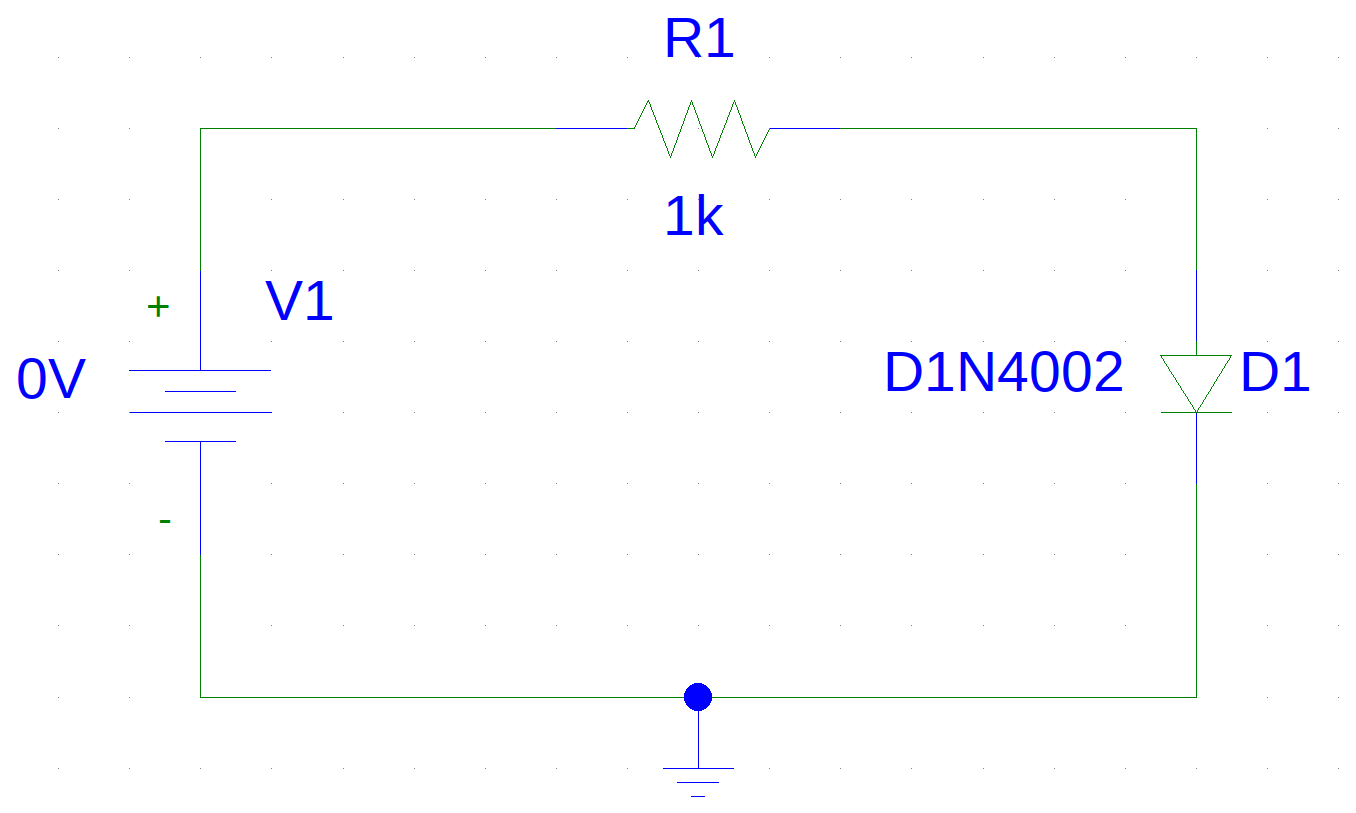
\includegraphics[width=0.5\linewidth]{../schematics/fig2}
	\caption{PSpice DC sweep circuit for the D1N4002 PN junction diode with a 1 k $\Omega$ series resistor}
	\label{fig:fig2}
\end{figure}
\subsubsection*{5.2 Zener Diode Forward- and Reverse-Bias Sweeps}
\begin{figure}[H]
	\centering
	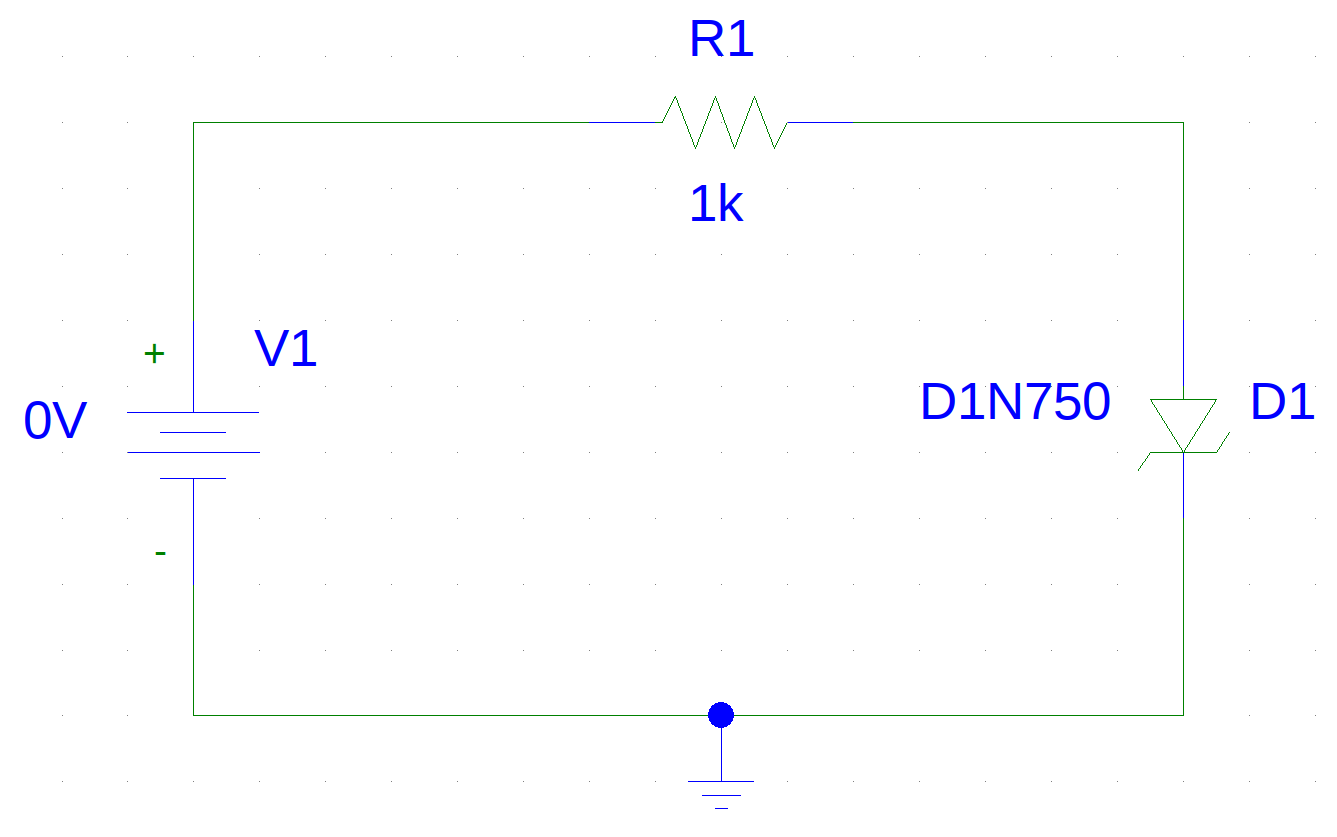
\includegraphics[width=0.5\linewidth]{../schematics/fig3}
	\caption{PSpice DC sweep circuit for the D1N750 Zener diode with a 1 k$\Omega$ current-limiting resistor.}
	\label{fig:fig3}
\end{figure}
\subsubsection*{5.3 Half-Wave Rectifier}
\begin{figure}[H]
	\centering
	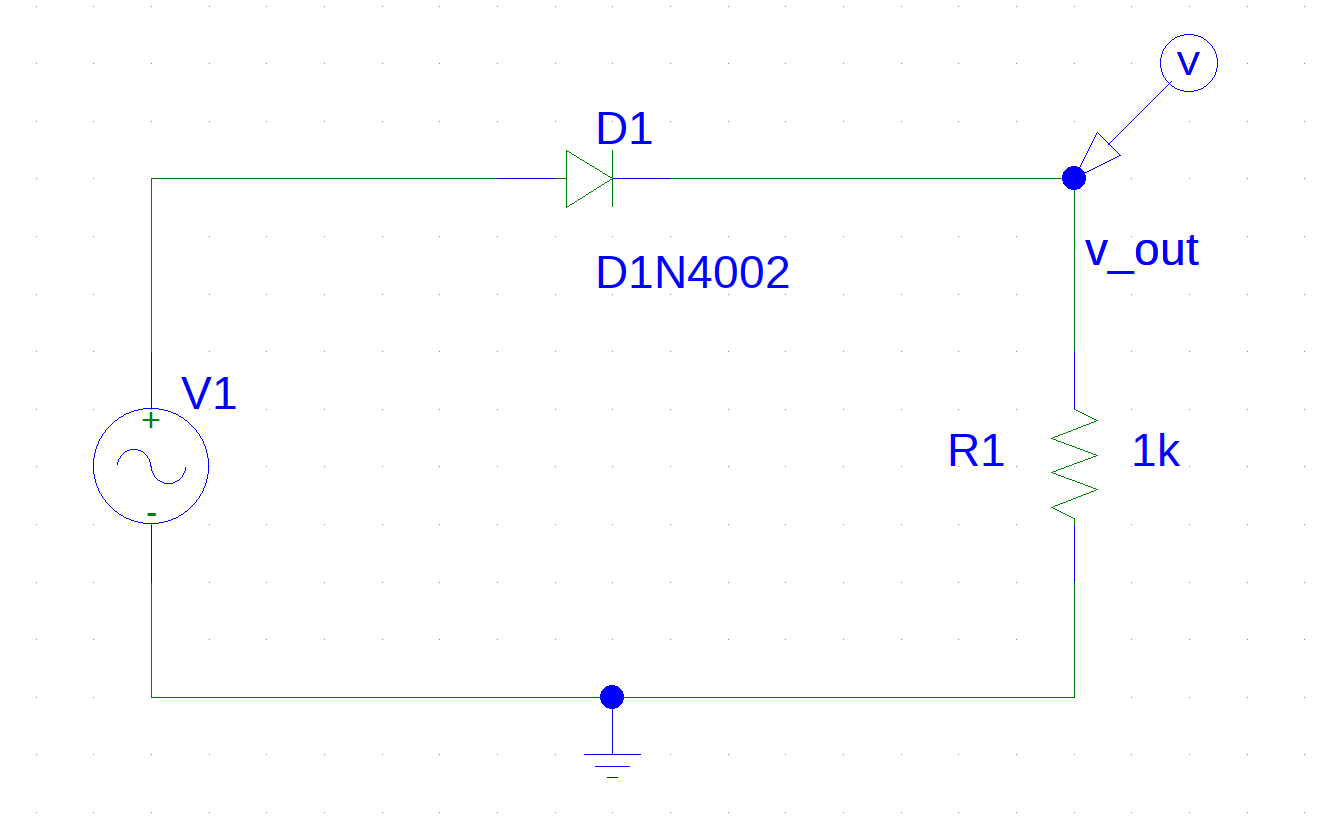
\includegraphics[width=0.5\linewidth]{../schematics/fig4}
	\caption{PSpice half-wave rectifier circuit used for the simulation.}
	\label{fig:fig4}
\end{figure}
\subsection*{7 Result Analysis}
\subsubsection*{7.1 PN Junction Diode Results}
\begin{figure}[H]
	\centering
	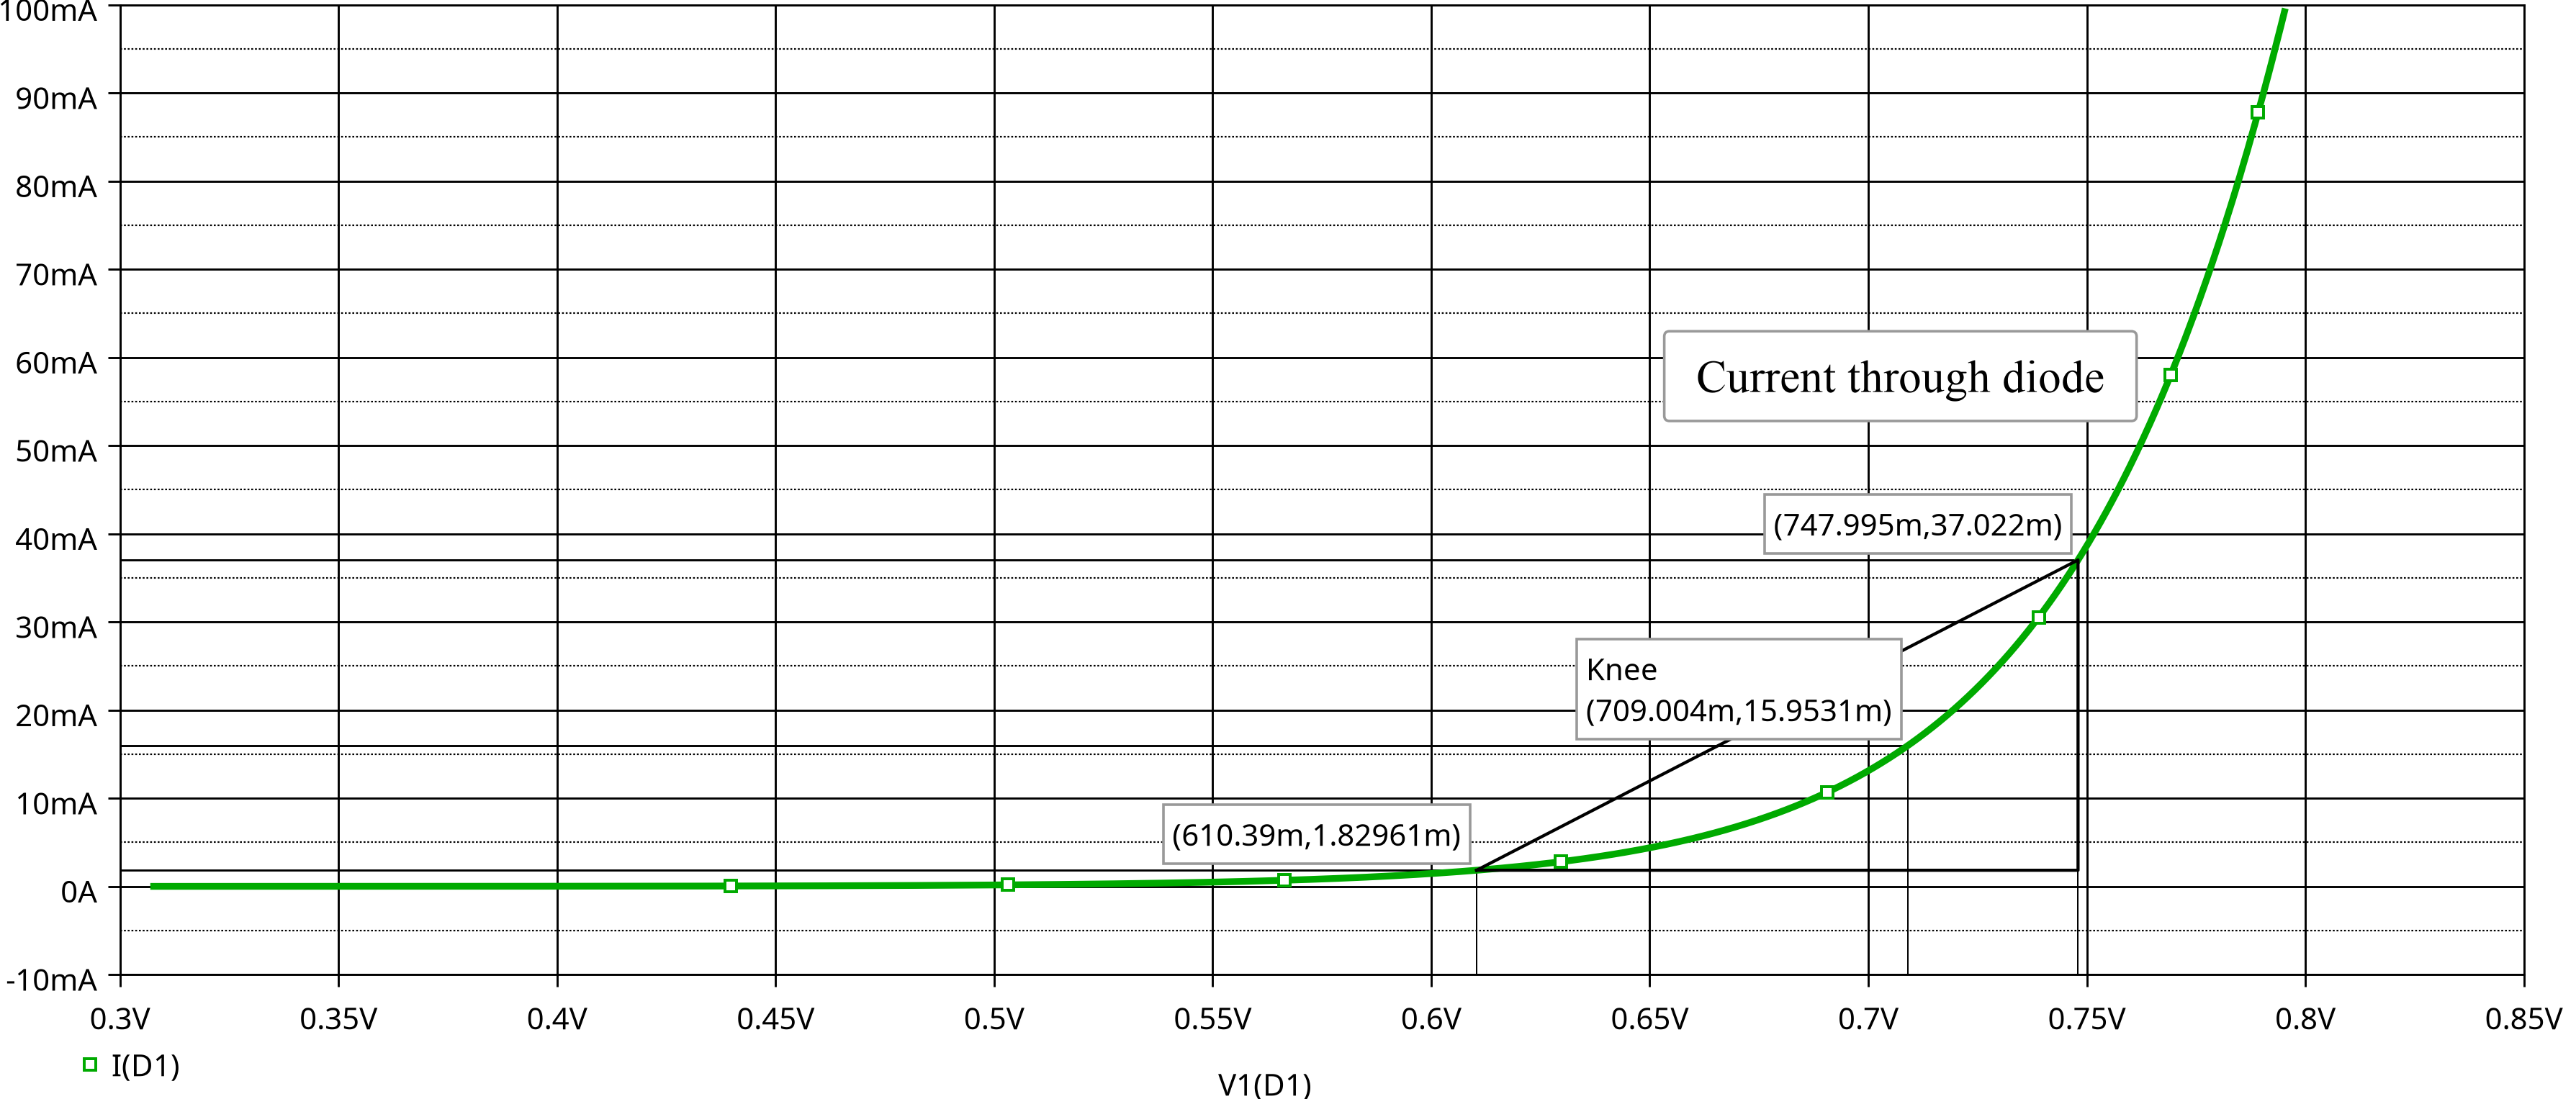
\includegraphics[width=0.9\linewidth]{../pspice_graphs/diode_forward_zoom}
	\caption{Forward-bias characteristic of the D1N4002 showing the knee region and selected cursor points.}
	\label{fig:diodeforwardzoom}
\end{figure}
\begin{figure}[H]
	\centering
	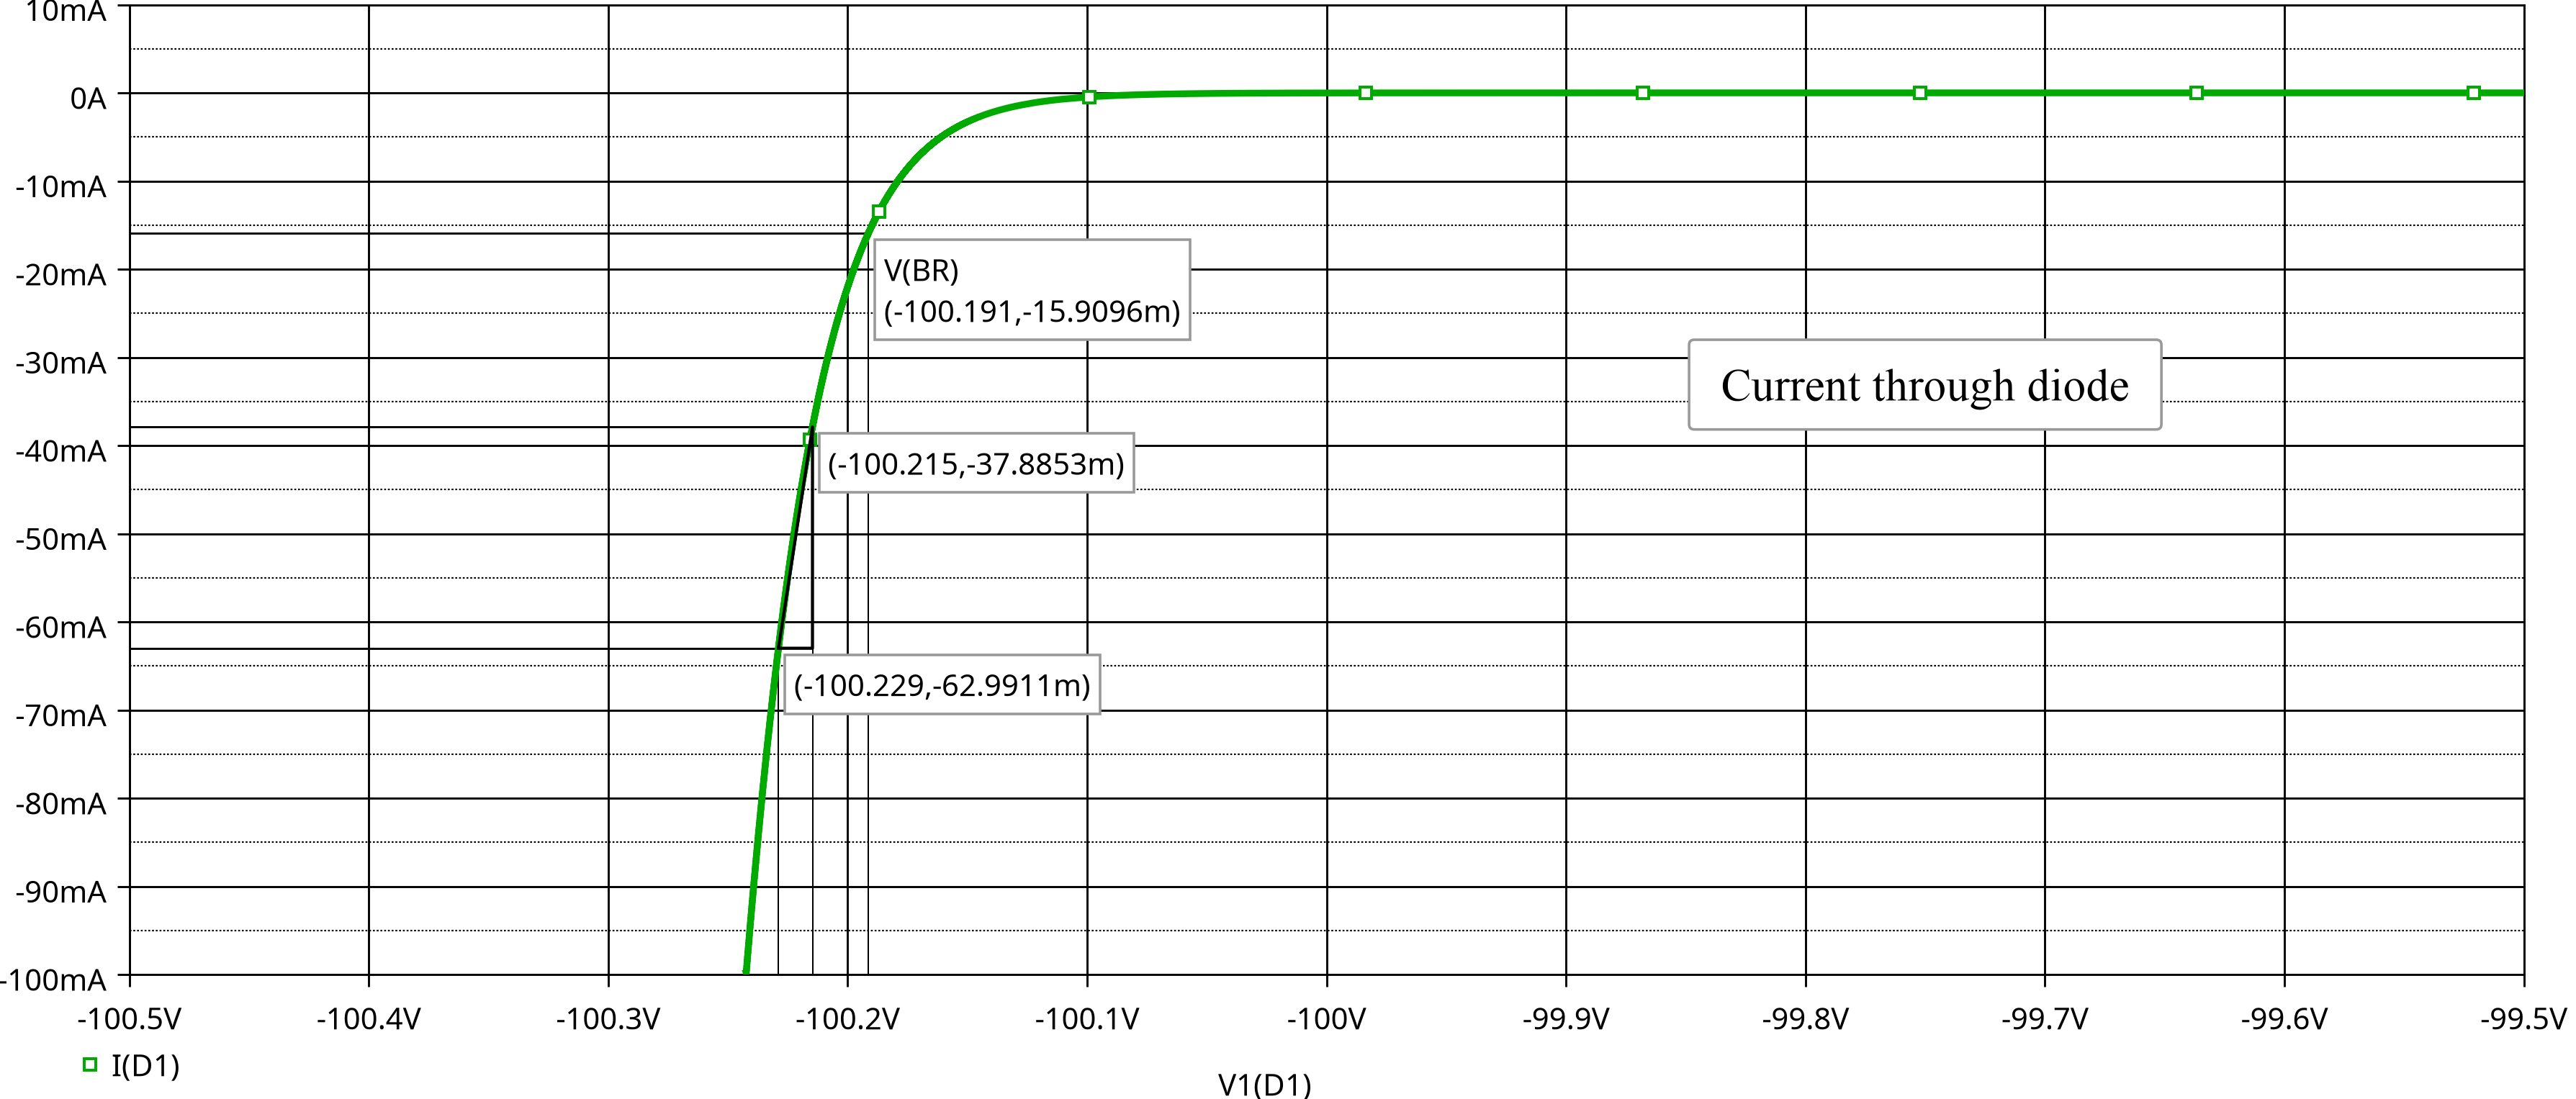
\includegraphics[width=0.9\linewidth]{../pspice_graphs/diode_reverse_zoom}
	\caption{Reverse-breakdown characteristic of the D1N4002 showing the selected cursor points.}
	\label{fig:diodereversezoom}
\end{figure}
\subsubsection*{7.2 Zener Diode Results}
\begin{figure}[H]
	\centering
	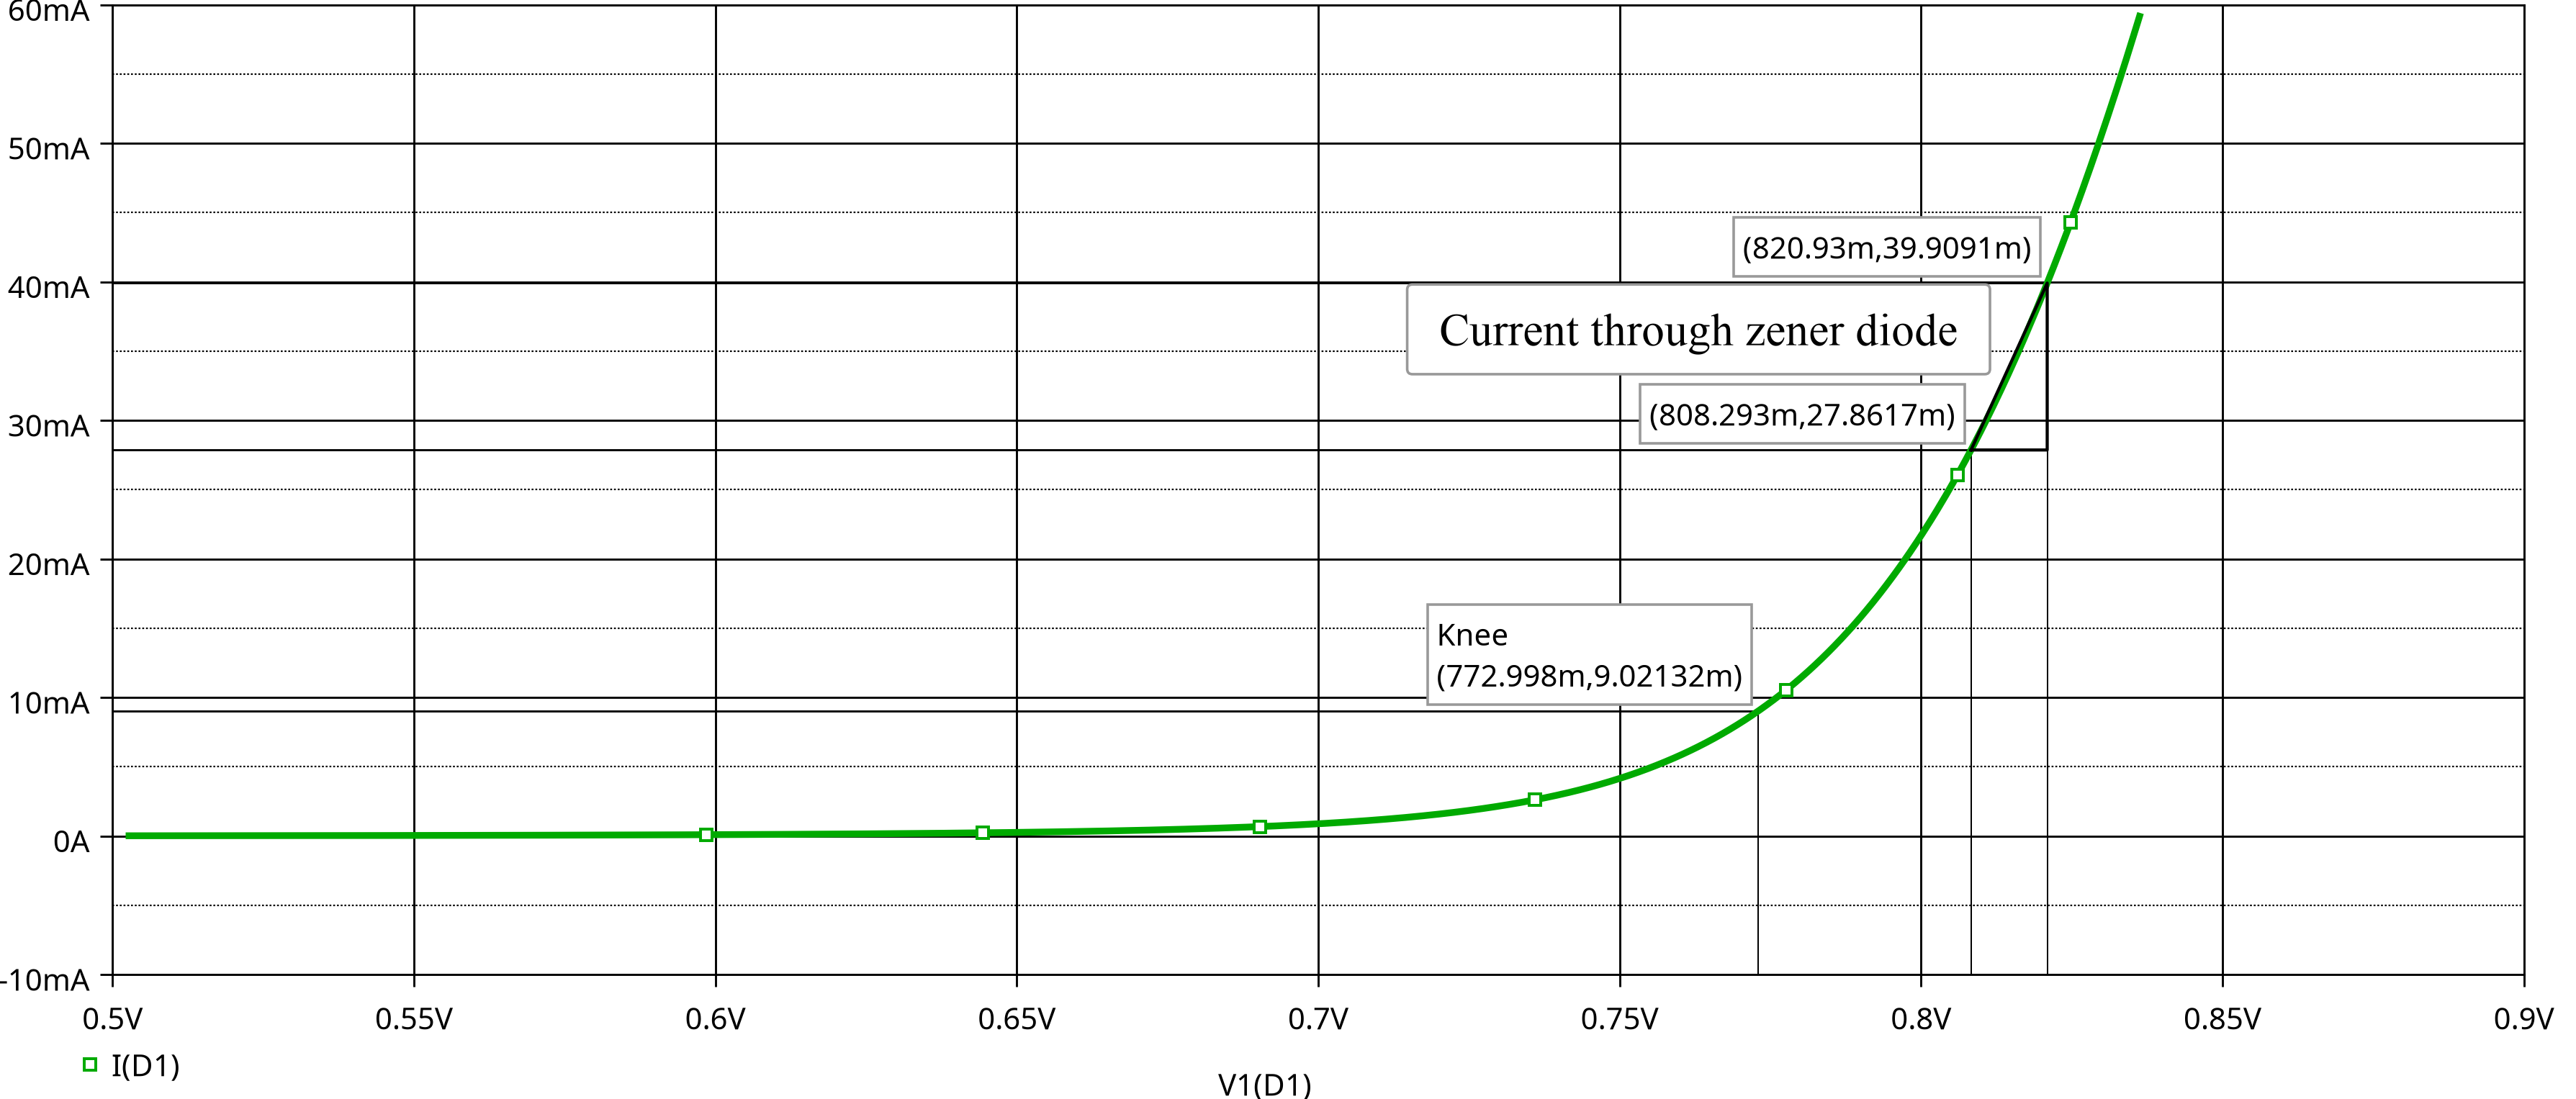
\includegraphics[width=0.9\linewidth]{../pspice_graphs/zener_forward_zoom}
	\caption{Forward-bias characteristic of the D1N750 Zener diode showing the knee region.}
	\label{fig:zenerforwardzoom}
\end{figure}
\begin{figure}[H]
	\centering
	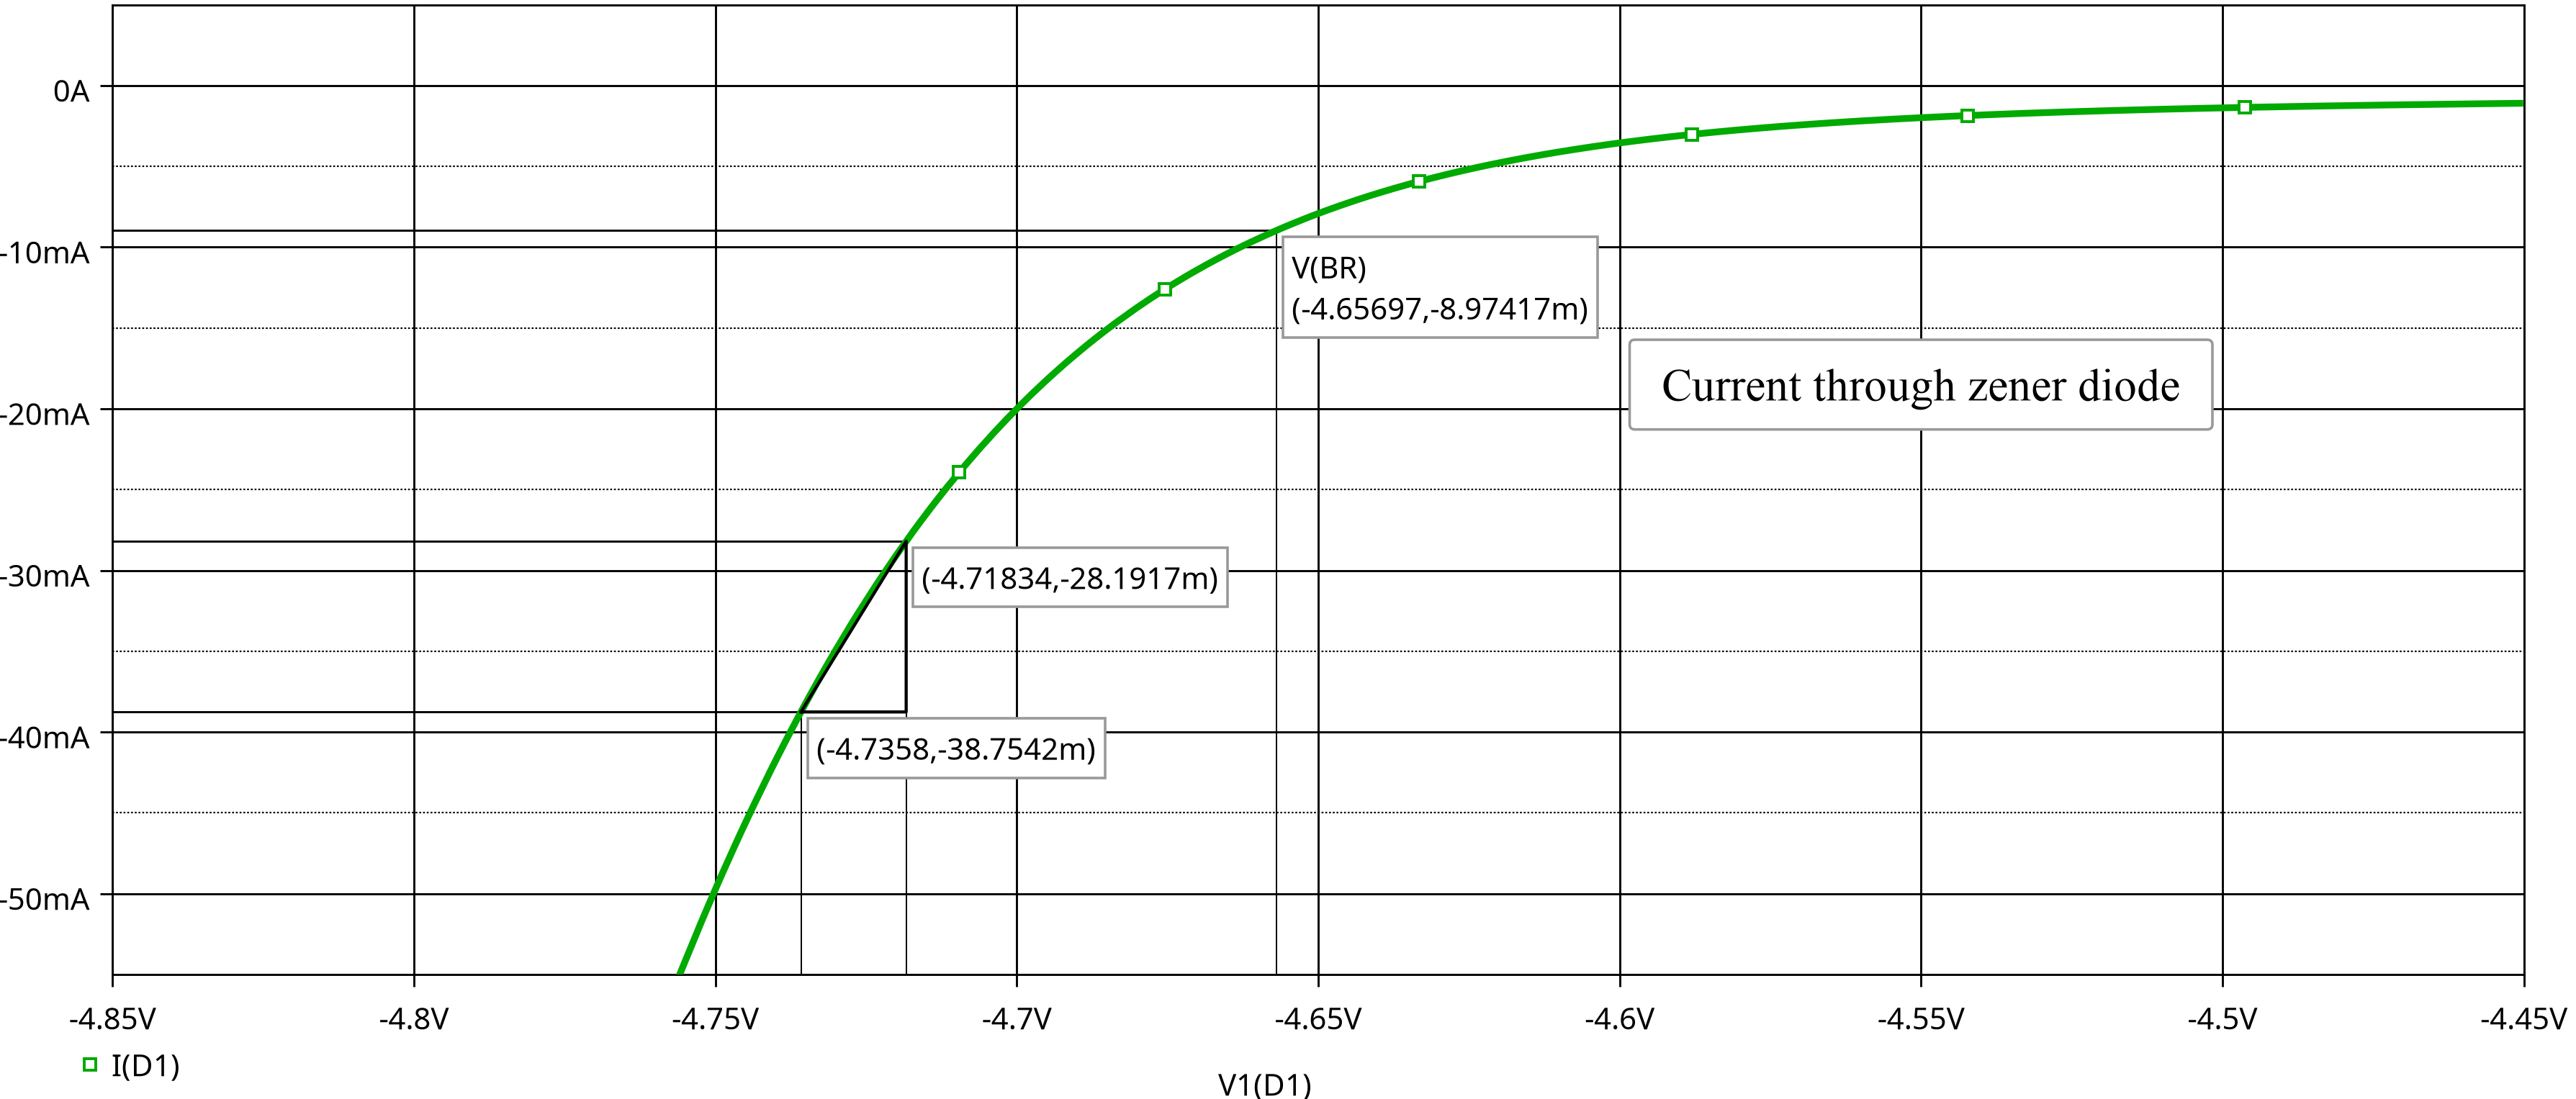
\includegraphics[width=0.9\linewidth]{../pspice_graphs/zener_reverse_zoom}
	\caption{Reverse-breakdown characteristic of the D1N750 Zener diode showing the selected cursor points.}
	\label{fig:zenerreversezoom}
\end{figure}
\subsubsection*{7.3 Half-Wave Rectifier Results}
\begin{figure}[H]
	\centering
	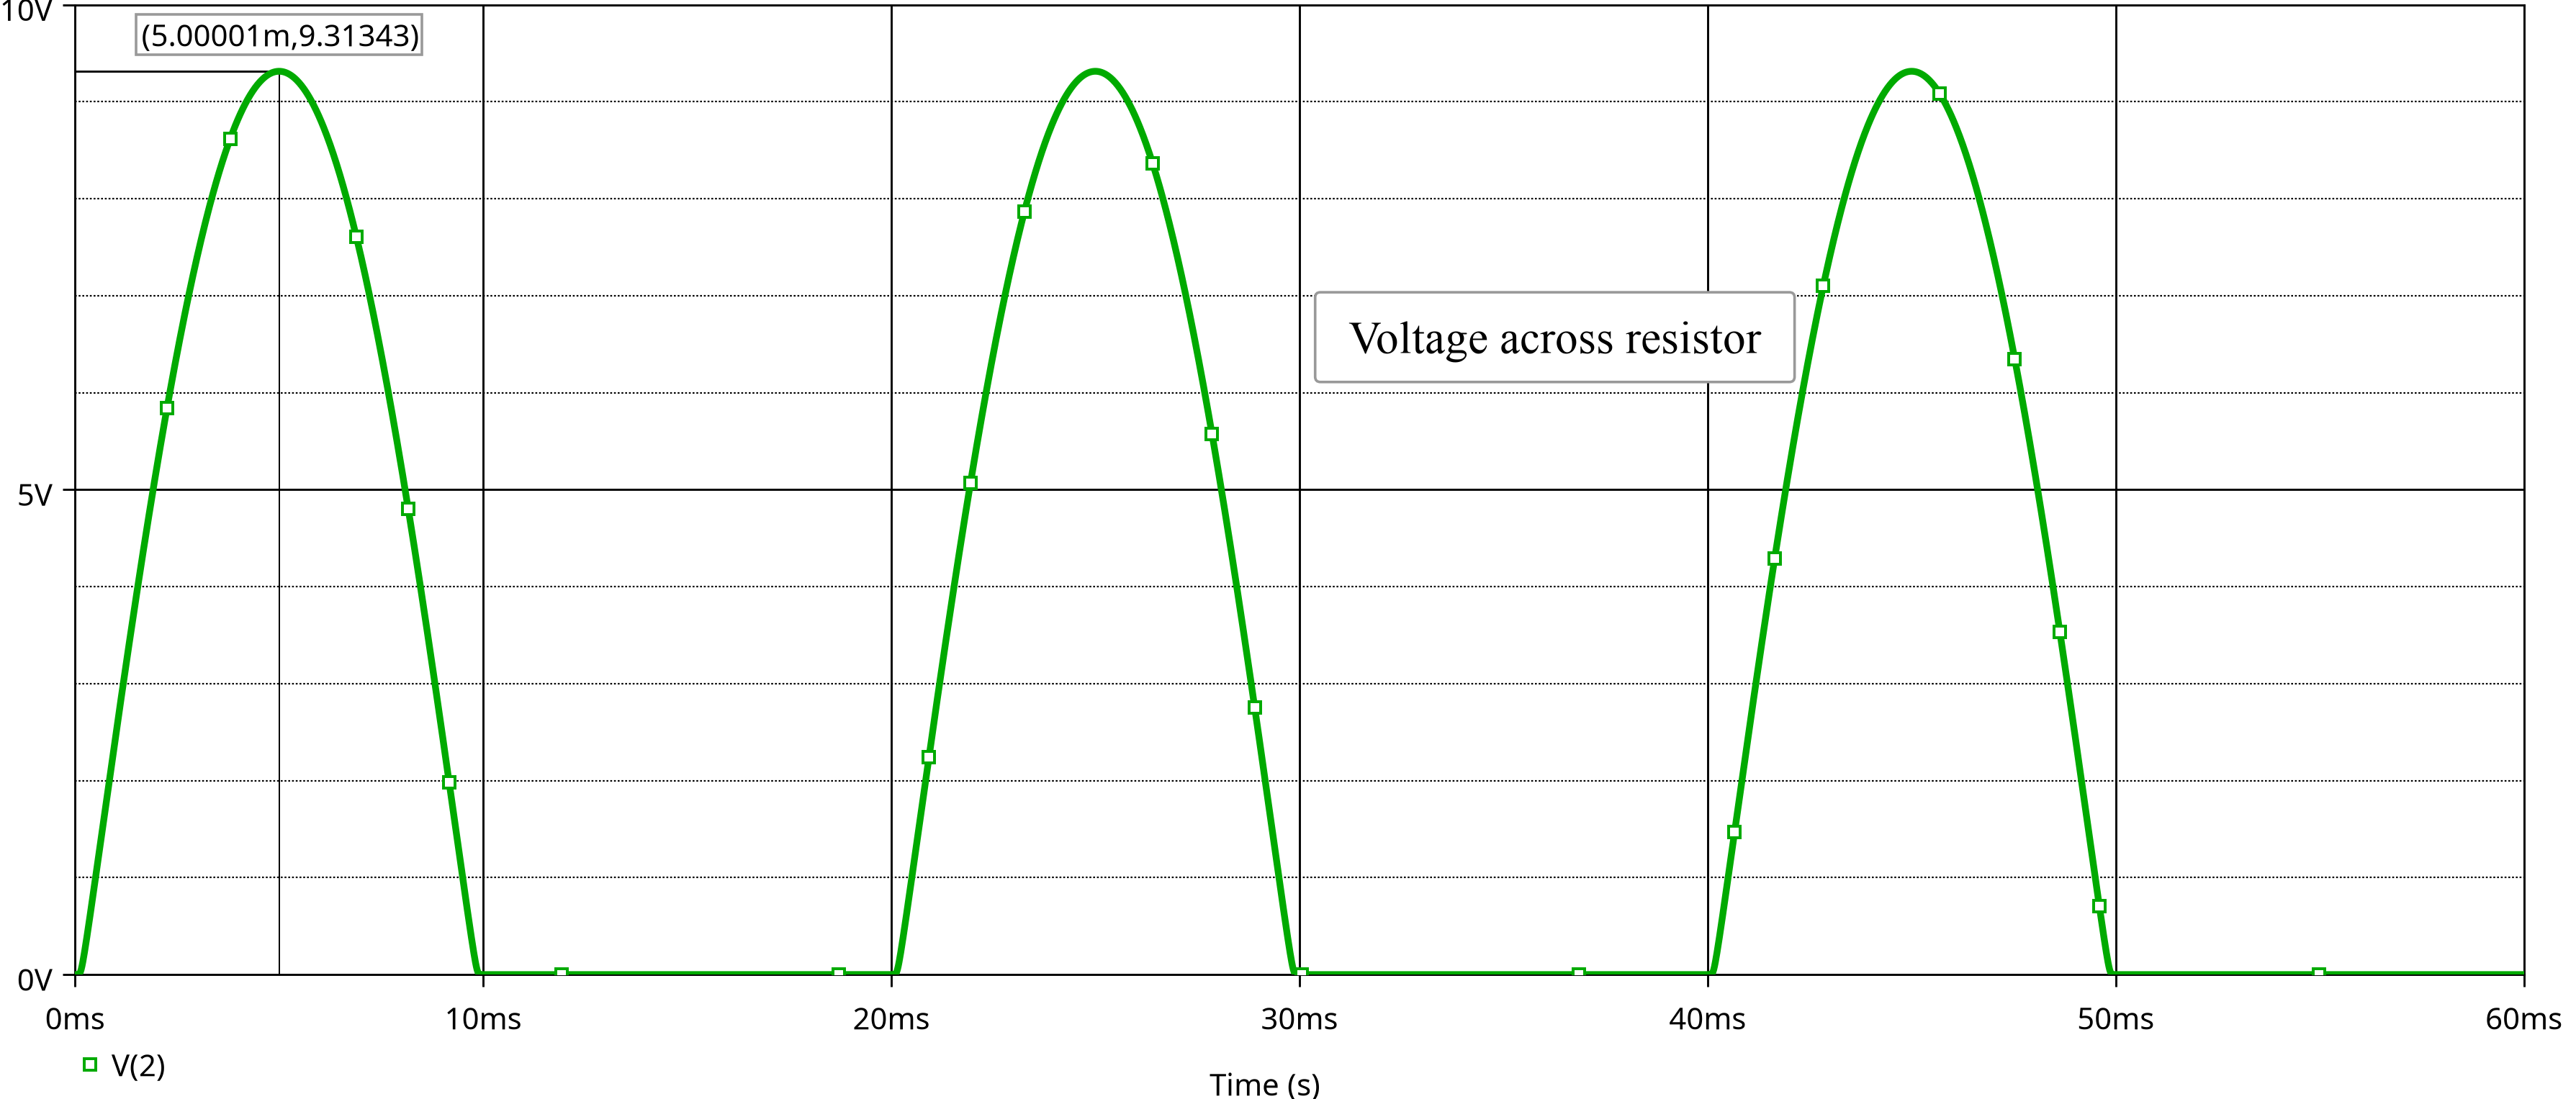
\includegraphics[width=0.9\linewidth]{../pspice_graphs/half_wave_rectifier}
	\caption{Simulated output-voltage waveform of the D1N4002 half-wave rectifier.}
	\label{fig:halfwaverectifier}
\end{figure}

\end{document}